\chapter{Séquence Stack-Of-Star UTE auto-synchronisée sur le rythme cardiaque combinée à l'injection de nanoparticules de fer}
\setlength{\footskip}{50pt}
\chaptermark{Angiographie cardiaque autosynchronisée}
\label{Chap5}
\section{Contexte}


La synchronisation sur le rythme cardiaque grâce aux électrodes ECG est la principale limitation de la méthode décrite dans le chapitre précédent. En effet, cette stratégie de synchronisation sur le rythme cardiaque est sensible aux interférences créé par les gradients de forte intensité nécessaires pour obtenir une imagerie haute résolution mais aussi aux problèmex de conduction cardiaque anormal qui peuvent apparaître dans certains modèles pathologiques. 
Durant ce travail de thèse nous avons été exposé à ces problèmatiques dans le cadre de l'imagerie d'un modèle de souris avec un infarctus aiguë du myocarde. Il a donc été nécessaire d'adapter la méthode d'imagerie anatomique précédente à ce type de modèle. 

L'approche employée a été d'utiliser une méthode d'auto-synchronisation sur le rythme cardiaque à partir des données brutes IRM. De nombreuses approches différentes sont présentées dans la littérature chez l'humain \cite{Liu:2010aa,Liu:2014ab,Ingle:2014aa,Pang:2014aa} ou le rat \cite{Kramer:2014aa} mais requiert des acquisitions de données supplémentaires. Cette méthode est difficilement exploitable chez la souris car le rythme cardiaque d'une souris anesthésiée est supérieur à 400 battements par minute. Il est donc nécessaire de recueillir les signaux servant pour l'auto-synchronisation régulièrement pour avoir une visualisation suffisante de la modification d'intensité du signal. Le rapport signaux d'auto-synchronisation et signaux utiles à la reconstruction d'image devient alors faible ce qui augmente considérablement le temps d'acquisition.

Une autre approche envisageable est l'utilisation d'un écho-navigateur pour chaque acquisition de signal qui permet d'obtenir une fréquence d'échantillonnage du signal égale au temps de répétition de la séquence. Le signal de l'écho-navigateur est recueilli au centre de l'espace de Fourier et est donc sensible au signal/constrate globale de l'image or celui-ci est modifié lorsque le coeur se contracte et il est donc possible de suivre les déformations cardiaques au cours du temps. Cette méthode a déjà était employé avec des séquences de type cartésienne \cite{Bovens:2011aa} ou radiale UTE \cite{Hoerr:2013gf,Motaal:2015aa} mais seulement pour des acquisitions 2D, cela s'explique par le fait que le signal d'écho-navigateur est plus sensible aux modifications lorsqu'il y a un fort contraste entre le sang et les autres tissus et est aisément visible en 2D avec le signal temps-de-vol.
Une seule publication fait état d'une méthode d'auto-synchronisation pour une acquisition 3D cardiaque chez la souris \cite{Nieman:2009aa} mais celle-ci requiert un temps d'acquisition supérieur à 2 heures difficilement compatible avec des études longitudinales sur des modèles pathologiques. De plus, des artéfacts de flux sont présent sur leurs images dû à la trajectoire cartésienne utilisée.

L'approche 3D nécessite donc d'augmenter le signal du sang dans le cas de l'imagerie cardiaque. L'étude du chapitre précédent a montré qu'il était possible d'utiliser des agents de contraste à base de nanoparticules de fer combinées avec des séquences à temps d'écho court pour obtenir un signal positif du sang. La séquence radiale UTE 3D peut sur le principe être utilisée en tant que séquence auto-synchronisée puisqu'il est possible d'utilisée le premier point qui est le même pour chaque projection comme écho-navigateur. Cependant l'impulsion de radiofréquence étant non-sélective, le champ de vue est important et la variation de signal provenant de la contraction cardiaque est alors trop faible en pourcentage par rapport au reste du signal. 

C'est pourquoi nous proposons dans ce travail d'utiliser une séquence de type stack-of-star UTE auto-synchroniser sur le rythme cardiaque en combinaison avec l'injection d'un agent de contraste à base de nanoparticules de fer. La trajectoire stack-of-star UTE permet d'utiliser une sélection de coupe pour le volume 3D comprenant seulement le coeur et donc permettant d'augmenter le pourcentage de signal venant de sa contraction par rapport au signal des autres tissus. La séquence sera utilisée pour permettre l'acquisition d'image avec une forte résolution spatiotemporelle sur un modèle de souris d'infarctus aiguë du myocarde.
%Cette séquence sera implémenté selon une trajectoire basé sur l'angle d'or 2D et son efficacité à remplir un espace de Fourier de manière uniforme sera comparé à la trajectoire incrémentale standard.

\section{Séquence Stack-Of-Star UTE auto-synchronisée sur le rythme cardiaque.}

\subsection{Chronogramme de la séquence}

La séquence Stack-Of-Star UTE combine une trajectoire UTE 2D à un encodage 3D cartésien dans la troisième dimension. Cette trajectoire fait apparaitre des artéfacts de type "streaking" du même type que ceux en 2D pour les forts facteurs de sous-échantillonnage comme illustré dans la figure \ref{fig:SoSUTE} mais elle permet de réduire le champ de vue dans la direction de coupe par rapport à la séquence UTE 3D. Cette propriété est nécessaire pour permettre d'obtenir une variation du signal suffisante provoquée par la contraction du coeur. Le deuxième point intéressant de cette trajectoire est son faible temps d'écho (inférieur à 600 $\mu s$) qui permet avec les concentrations de nanoparticules de fer injectées d'obtenir un contraste positif. De plus cela permet aussi d'obtenir des images moins impactée par les artéfacts de déphasage de flux par rapport à une séquence cartésienne \cite{Hoerr:2013gf}.

\begin{figure}[H]
\centering
\line(1,0){400} \\
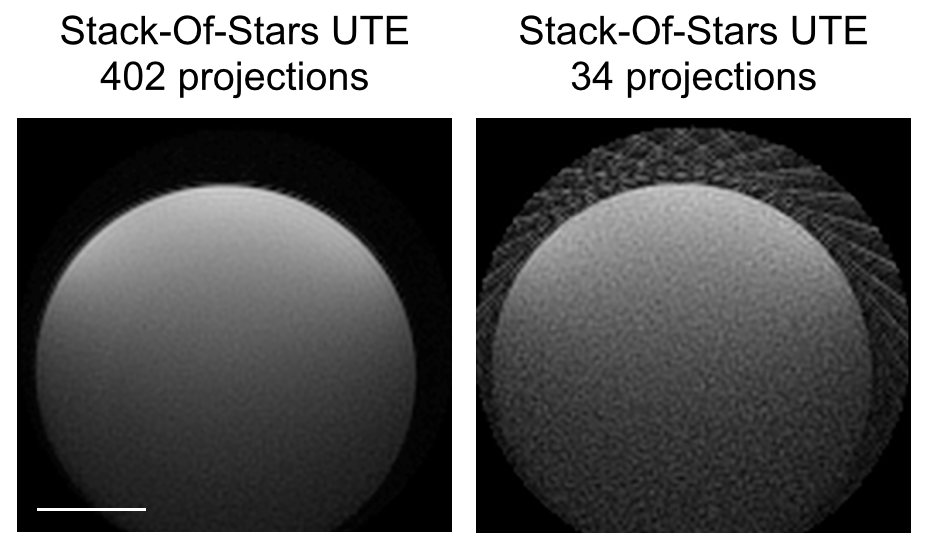
\includegraphics[scale=0.5]{./figure/chap5/Fig1.png}
\caption[Effet du sous-échantillonnage SoSUTE]{\label{fig:SoSUTE} Images obtenue sur un fantôme d'eau avec une séquence Stack-Of-Star UTE avec 402 projections à gauche et 34 projections à droite. On observe des artéfacts de "streaking" particulièrement visible en dehors du fantôme. La barre d'échelle mesure 7,5 mm.}
\line(1,0){400} \\ 
\end{figure}

La séquence a été modifiée pour permettre de recueillir un signal d'écho-navigateur. Généralement, les gradients de rephasage de coupe et de codage de phase dans la direction de coupe sont appliqués en même temps. Ici, les deux gradients sont séparés pour permettre de recueillir le signal d'écho-navigateur durant le gradient de rephasage de coupe donc au centre de l'espace de Fourier. Le nombre de point à recueillir, indiqué en vert sur la figure \ref{fig:SeqSoSUTE}, peut être modifié pour accumuler le signal.

Les trajectoires utilisées dans ce travail sont définies selon la méthode incrémentale $\Phi = i \times \frac{360\degres}{N_p}$ et le golden angle 2D $\Phi = i \times 222.48\degres mod(360\degres)$ où $N_p$ est le nombre de projection par partition selon la direction de coupe. Toutes les projections d'une partition sont recueillies avant le passage vers la partition suivante.

La méthode employée ici étant une stratégie de reconstruction rétrospective, ce schéma d'acquisition est répété un nombre de fois égale au nombre de répétition NR. Lors de cet article les données ont été recueillies avec un nombre ${NR}=10$ puis sous-échantillonnée a posteriori pour évaluer la robustesse de l'acquisition au sous-échantillonnage.

\begin{figure}[H]
\centering
\line(1,0){400} \\
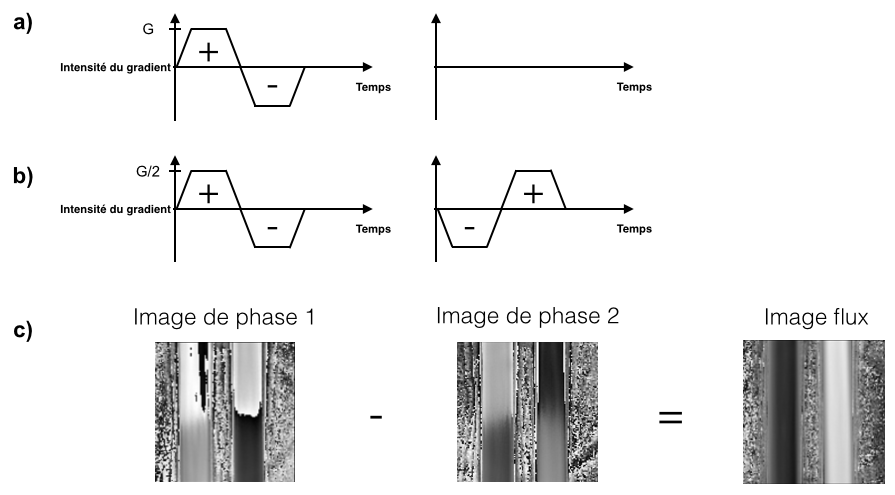
\includegraphics[scale=0.5]{./figure/chap5/Fig2.png}
\caption[Séquence auto-synchronisée]{\label{fig:SeqSoSUTE} Chronogramme de la séquence Stack-Of-Star UTE auto-synchronisée sur le rythme cardiaque. Le signal d'écho-navigateur (en vert) est recueilli durant le gradient de rephasage de coupe. Le signal utilisé pour la reconstruction est indiqué en rouge est est encodé selon une trajectoire incrémentale ou d'angle d'or 2D.}
\line(1,0){400} \\ 
\end{figure}

\subsection{Traitement du signal d'écho-navigateur.}

Le signal d'écho-navigateur est utilisé pour extraire les mouvements de contraction du coeur. Les points recueillis sont additionnés de manière complexe pour chaque projection. Le signal est convolué avec un filtre gaussien pour limiter les effets du bruit sur la détection des pics (voir figure \ref{fig:Signal}). L'écart médian entre les pics ainsi que son écart type sont calculés et permettent de ne pas utiliser les données entre deux pics détectés s'ils sont distants de plus 2 fois l'écart type par rapport à la valeur médiane.

Le nombre de volume ciné (NCiné) reconstruit durant le mouvement cardiaque est défini par l'utilisateur. Les données sont regroupées en fonction de leurs positions relatives entre deux pics de l'écho-navigateur dans les espaces de Fourier correspondant au cycle cardiaque permettant ensuite de reconstruire les volumes cinés avec la procédure de reconstruction "gridding" évoqué dans le chapitre \ref{Chap2}.

Des exemples de signaux écho-navigateur sont montrés dans la figure \ref{fig:Signal} pour une acquisition 2D et 3D sans injection de produit de contraste et après injection de 200 $\mu mol Fe/kg$. Le signal écho-navigateur 2D (figure \ref{fig:Signal}.a) est parfaitement exploitable grâce à l'effet temps-de vol qui permet d'obtenir un fort signal du sang et donc de visualiser la contraction du coeur grâce à la diminution du signal provenant des ventricules. En 3D, avant injection (figure \ref{fig:Signal}.b), le signal écho-navigateur est fortement bruité ce qui a pour effet de limiter la détection des pics avec les données brutes cependant après l'utilisation du filtre gaussien, les pics peuvent être extraits. Après injection  de l'agent de contraste (figure \ref{fig:Signal}.c), le signal écho-navigateur est rehaussé ainsi que sa variation relative, ceci s'explique par l'augmentation globale du signal sanguin qui peut s'observer sur les images axiales du coeur.

\begin{figure}[H]
\centering
\line(1,0){400} \\
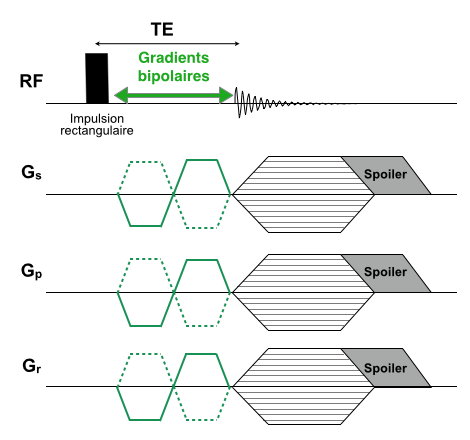
\includegraphics[scale=0.5]{./figure/chap5/Fig3.png}
\caption[Signal d'écho-navigateur]{\label{fig:Signal} Schéma présentant le signal écho-navigateur cardiaque obtenu durant une acquisition sur une souris avec une séquence \textbf{(a)} UTE 2D sans injection et \textbf{(b)}Stack-Of-Star UTE 3D avant injection et \textbf{(c)} après injection de 200 $\mu mol Fe/kg$. Le signal brut est présenté sur le schéma du haut et après convolution avec un filtre gaussien sur le schéma du bas. Les images axiales du coeur correspondantes sont présentée en bas. La barre d'échelle mesure 5 mm.}
\line(1,0){400} \\ 
\end{figure}

\section{Répartition des projections incrémentale ou selon l'angle d'or 2D.}

Dans le cas d'une reconstruction rétrospective la méthode de répartition des projections au cours du temps a une influence sur le résultat. Par exemple dans le cas de la suppresion des projections corrompues par la respiration, avec une trajectoire incrémentale une partie de l'espace de Fourier n'est pas rempli car les projections sont adjacentes alors qu'avec une trajectoire aléatoire, ces suppressions de projection sont réparties dans tout l'espace de Fourier et non pas centralisée autour d'une position.

Pour valider cette affirmation dans le cas d'une séquence cardiaque 3D, deux paramètres ont été étudiés : L'angle moyen et l'écart type entre les projections les plus proches dans chaque partition. Les données de synchronisation sont extraites à partir du signal écho-navigateur \textit{in vivo} d'acquisitions réalisées sur 4 animaux différents. Ces données sont alors traitées en utilisant les deux types de trajectoires pour en extraire l'angle moyen et l'écart-type. Ces paramètres ont été calculés en sous-échantillonant a posteriori les données acquises de $NR = 10$ à $NR = 1$ et avec $NCine = 10$ et un nombre de projection par partition $NProj = 402$.
L'angle moyen minimum qui peut être obtenu en fonction du NR est égale à $\frac{360\degres \times NCine}{NProj \times NR}$ ce qui donne  (0,90; 1,00; 1,12; 1,28; 1,49; 1,79; 2,24; 2,99; 4,48; 8,96) degrés pour les valeurs de NR de 10 à 1.

\begin{figure}[H]
\centering
\line(1,0){400} \\
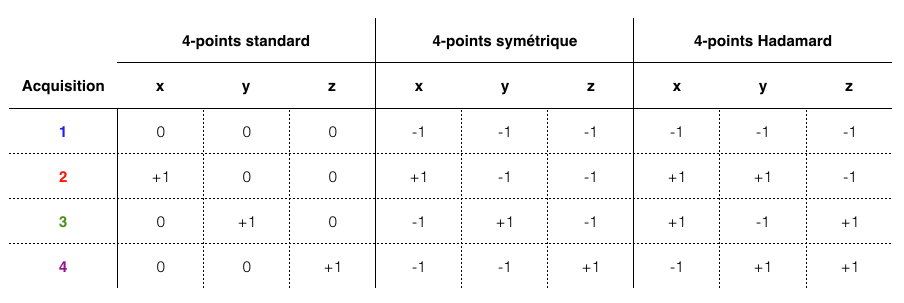
\includegraphics[scale=0.4]{./figure/chap5/Fig4.png}
\caption[Influence de la trajectoire en fonction du sous-échantillonnage]{\label{fig:GoldVSIncNr} Graphique représentant \textbf{(a)} la moyenne et \textbf{(b)} l'écart-type des angles entre les projections les plus proches dans une même partition en fonction du nombre de NR utilisé pour la reconstruction. Les paramètres sont affichés pour la répartition incrémentale des projections et selon l'angle d'or 2D.}
\line(1,0){400} \\ 
\end{figure}

Les valeurs calculés sont représentées dans la figure \ref{fig:GoldVSIncNr}. On observe que les valeurs d'angle moyen sont équivalentes entre la méthode incrémentale et d'angle d'or 2D, bien qu'elle soit légérement supérieure avec la méthode incrémentale. Quel que soit la valeur NR, l'angle moyen est supérieur à la répartition idéale des projections ce qui s'explique par l'aspect rétrospectif et non pas prospectif de l'acquisition qui ne permet pas de recueillir toutes les projections dans chaque partition. 
La différence entre les deux méthodes de répartition des projections s'observe sur les valeurs des écarts-types. Quelles que soient les valeurs de NR, la répartition avec l'angle d'or 2D permet d'obtenir un écart-type plus faible que la répartition incrémentale. Cela traduit une meilleure homogénéité de la répartition des projections dans les partitions.
Ce résultat est aussi visible sur les images, on observe sur la figure \ref{fig:ImGoldVSIncNr} une diminution en terme de qualité des images en fonction de la valeur NR plus rapide pour la répartition incrémentale. Cela est particulièrement visible à partir de $NR = 4$ où la délimitation du myocarde est plus floue en particulier dans l'orientation axiale.
 
\begin{figure}[H]
\centering
\line(1,0){400} \\
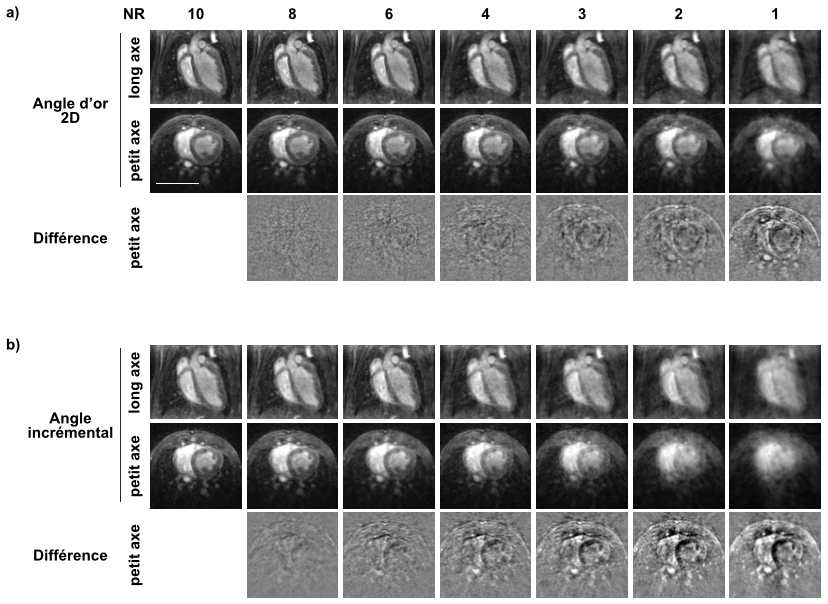
\includegraphics[scale=0.4]{./figure/chap5/Fig5.png}
\caption[Image de l'nfluence de la trajectoire en fonction du sous-échantillonnage]{\label{fig:ImGoldVSIncNr} Images axiales et coronales d'un coeur de souris saine reconstruite avec un nombre décroissant de nombre de répétition (NR) avec une répartition incrémentale et avec l'angle d'or 2D. La barre d'échelle mesure 10 mm.}
\line(1,0){400} \\ 
\end{figure}

La flexibilité de cette méthode d'auto-synchronisation permet de modifier le nombre de volumes cinés reconstruites à partir d'un même jeu de donnée. La figure \ref{fig:GoldVSIncNCine} montre l'écart-type en fonction du nombre de volumes cinés reconstruits pour plusieurs valeurs NR. L'écart-type est plus faible dans la plupart des cas avec la méthode de répartition d'angle d'or 2D. L'écart entre les valeurs obtenues avec la répartition incrémentale et d'angle d'or 2D diminue avec l'augmentation du nombre de volumes cinés reconstruits et l'on observe un croisement des courbes pour les valeurs de paramètres : NR < 6 et NCine = 30 bien que les différences entre les deux courbes ne soient pas significatives. Cependant, il est a noté que les cas où les courbes se croisent sont des cas extrêmes qui ne permettent pas d'obtenir des images de bonne qualité à cause de l'utilisation d'un facteur de sous-échantillonnage trop important.

Ces différentes observations justifient l'utilisation de l'angle d'or 2D pour répartir les projections puisque celle-ci permet une répartition plus homogène pour un large choix de valeur des paramètres (NCine, NR). 

\begin{figure}[H]
\centering
\line(1,0){400} \\
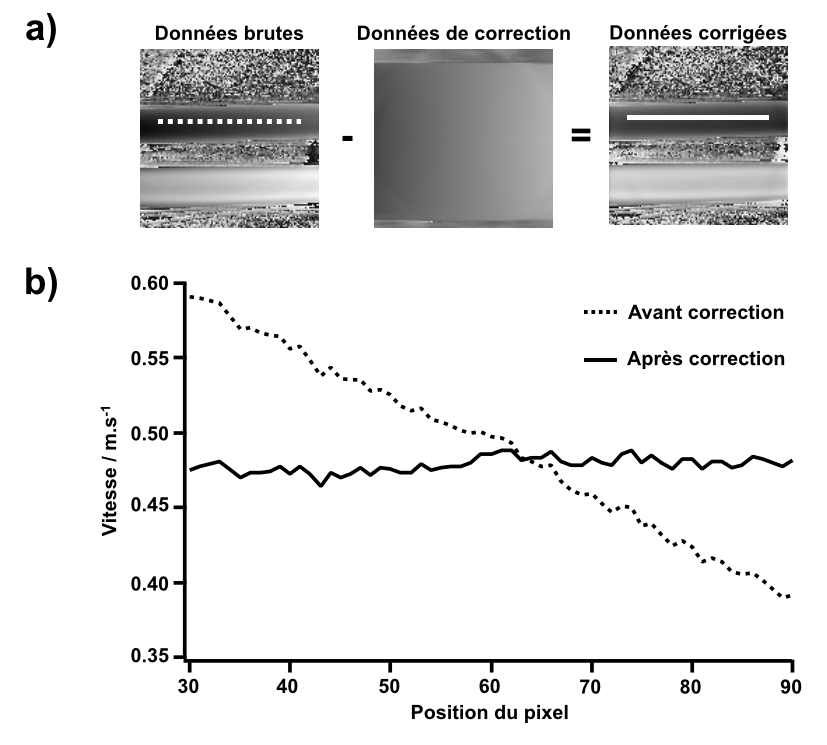
\includegraphics[scale=0.4]{./figure/chap5/Fig6.png}
\caption[Influence de la trajectoire en fonction du nombre d'images cinés reconstruite]{\label{fig:GoldVSIncNCine} Graphique représentant  l'écart-type des angles entre les projections les plus proches dans une même partition en fonction du nombre de volumes cinés reconstruits pour la répartition incrémentale et selon l'angle d'or 2D. Les mesures sont représentées en fonction de nombre du nombre de répétition (NR) utilisé pour la reconstruction.}
\line(1,0){400} \\ 
\end{figure}

\section{Imagerie d'un modèle de souris d'infarctus du myocarde aiguë}

L'imagerie des souris a été effectué à 7 Tesla avec une antenne surfacique à 4 éléments. Les paramètres d'acquisitions sont les suivants :
TR/TE = 4.5/0.527 ms, type d'excitation radiofréquence/durée/angle d'excitation = hermite/0,3 ms/15$\degres$, champ de vue = 20 x 20 x 20, matrice = 128 x 128 x 128, nombre de partition = 96, nombre de projection par partition = 402, bande passante de réception = 100 kHz, nombre de répétition = 10, temps d'acquisition total : 25 minutes, 3 points recueillis pour l'écho-navigateur.

8 souris OF1 ont été imagées, séparées en un groupe sain et un groupe avec un infarctus aiguë du myocarde. Les souris ont été injectées avec un volume de 150 $\mu L$ de Sinerem (Guerbet, Aulnay-sous-bois, France) à une concentration de 200 $\mu mol$ Fe/kg avant le positionnement dans l'imageur.

\subsection{Qualité des images}

Des images représentatives obtenues sur une souris pathologique avec une résolution par pixel de 156 $\mu m$ isotropique sont montrées sur la figure \ref{fig:ImInfarct}. L'injection de l'agent de contraste permet de rehausser le signal du sang dans tout le volume et permet d'obtenir un bon rapport signal-sur-bruit du sang dans les ventricules égal à $36,5 \pm 5,3$ bien que le TE soit supérieur à 0,5 ms. Le contraste obtenu entre le myocarde et le sang est aussi important ($20,7 \pm 0,7$) et permet de parfaitement segmenter le myocarde pour extraire les paramètres fonctionnels. Il est à noter que les images présentent peu d'artéfacts normalement provoqués par le déphasage des flux et cela même durant la phase systolique du coeur. Cependant, on observe sur certaines acquisitions la présence d'un signal hyper intense dans l'oreillette droite dont l'intensité varie au cours du cycle cardiaque. Cet hyper signal est provoqué par un effet temps-de-vol qui n'est pas présent dans le sang sur le reste du l'image dû à la saturation des spins en imagerie cardiaque 3D.

\begin{figure}[H]
\centering
\line(1,0){400} \\
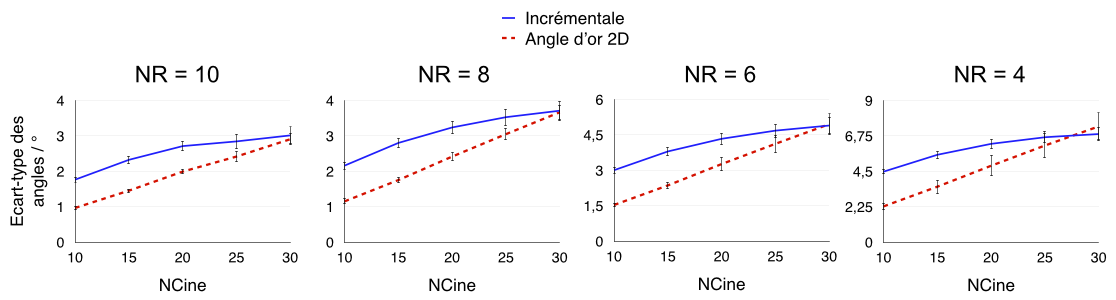
\includegraphics[scale=0.4]{./figure/chap5/Fig7.png}
\caption[Images obtenus sur une souris pathologique]{\label{fig:ImInfarct} Images coronales d'une acquisition représentative obtenue sur une souris pathologique. A gauche : Les images sont reconstruites avec des valeurs de paramètre NR = 6 et NCine = 10. A droite : NR = 10 et NCine = 20. La flèche blanche montre une partie avec un signal hyper-intense du sang dans l'image provoqué par l'effet temps-de-vol de la sélection de coupe. La barre d'échelle mesure 5 mm.}
\line(1,0){400} \\ 
\end{figure}

\subsection{Quantification de la fonction cardiaque.}

Le fort signal et contraste sur bruit des images permet d'obtenir une mesure précise du volume cardiaque, de la fonction cardiaque et de l'épaisseur du myocarde.
BLABLABLABLABLABLABLABLABLABLABLABLABLABLABLABLABLABLABLABLABLABLABLABLABLABLABLABLABLABLABLABLABLABLABLABLABLABLABLA
BLABLABLABLABLABLABLABLABLABLABLABLABLABLABLA

\section{Discussion}

L'imagerie 3D synchronisée prospectivement sur le rythme cardiaque demande une certaine expérience en terme d'expérimentation en particulier chez le petit animal. En effet, la qualité des images est dépendante du placement des électrodes pour obtenir un signal ECG suffisant en présence de gradient très intense ainsi que de la capacité à stabiliser le rythme cardiaque de l'animal durant l'acquisition. L'utilisation d'une séquence auto-synchronisé sur le rythme cardiaque grâce à l'utilisation d'un signal d'écho-navigation s'est donc avéré important. Une séquence Stack-Of-Star a donc été développé permettant l'acquisition d'un signal écho-navigateur à chaque TR et donc d'extraire un indicateur de la déformation du myocarde avec une fréquence élevée (supérieur à 200 Hz).

Bien que le TE minimum de la séquence Stack-Of-Star UTE soit supérieur à celui de la séquence UTE 3D présentée dans le chapitre précédent, celui reste toutefois faible par rapport aux séquence cartésienne classique. En effet, les acquisitions ont été effectuée avec des TE de 0,527 ms permettant de limiter suffisamment la décroissance du signal provoquée par l'effet $T_2^*$ des nanoparticules et donc d'obtenir un rehaussement positif du sang. Contrairement à la séquence UTE 3D, le signal ne croit avec la concentration en agent de contraste dans le sang mais atteint un maximum avant de diminuer. Cette concentration injectée peut être optimisée en fonction du temps d'écho de la séquence mais le fait de travailler \textit{in vivo} rend cette optimisation compliquée car la concentration effective d'agent de contraste dans le sang est difficile à estimer. La concentration utilisée dans cette étude est la même que celle de l'étude précédente car celle-ci permet d'obtenir un temps de demi-vie suffisamment long pour des acquisitions cardiaques. De plus, la gamme de concentration utilisée a été vérifiée par simulation puis \textit{in vivo} pour obtenir un rehaussement du signal suffisant pour l'application désirée. 
Ce rehaussement de signal permet d'utiliser des séquences en 3D dimensions qui permettent d'obtenir des mesures anatomiques ou fonctionnelles plus précises que les séquences 2D. En effet les séquences 3D ne requièrent pas de positionnement des coupes ce qui peut être particulièrement délicat dans le cas de modification de la forme du coeur pour certains modèles pathologiques \cite{Friedrich:2000aa,Sheehan2008Three-dimension}. De plus, l'extraction du signal d'écho-navigation est aussi amélioré grâce à l'injection de l'agent de contraste par rapport à une séquence 3D sans injection.

Les valeurs de contraste-sur-bruit obtenues avec cette méthode sont similaires à celles reportées dans la littérature \cite{Hoerr:2013gf,Motaal:2015aa} mais l'utilisation d'une acquisition 3D permet d'obtenir une résolution spatiale selon la direction de coupe 6 fois supérieure. De plus le temps d'acquisition par coupe/partition est aussi fortement réduit par rapport aux stratégies utilisant une séquence 2D UTE et cela même lorsqu'elles sont combinées à une reconstruction de type "compressed sensing" \cite{Motaal:2015aa}. Ce point est particulièrement intéressant car il permet de couvrir des zones étendues avec une forte résolution dans un temps d'acquisition raisonnable or dans certains modèles pathologiques le coeur peut subir des dilatations et demander un champ de vue  important.

L'autre avantage de l'utilisation d'une séquence Stack-Of-Star UTE est sa faible sensibilité aux artéfacts de mouvements et de flux ce qui permet d'obtenir un signal du sang très homogène même aux endroits enclin aux flux turbulents et ceci tout au long du cycle cardiaque. Cette propriété a déjà été montrée par Khadbi et al. \cite{Kadbi:2014uq} dans le cas d'une séquence de mesure de flux sur des fantômes de modèle sténotique.

Récemment, un intérêt pour l'angle d'or 2D a été montré pour des acquisitions 2D auto-synchronisés sur le rythme cardiaque que ce soit chez l'humain \cite{Kramer:2014aa,Kolbitsch2014Cardiac-functio} ou sur le rat \cite{Kramer:2013aa}. Cette trajectoire permet une plus grande grande flexibilité permettant par exemple d'obtenir des images temps-réel ou rétrospective à partir de la même acquisition. Dans cette étude, l'utilisation de angle d'or 2D a été étendue à une acquisition 3D sur le petit animal et permet une répartition plus homogène des projections que la méthode incrémentale classique. C'est pourquoi cette méthode est extrêmement flexible car elle permet une flexibilité lors de la reconstruction permettant l'optimisation ou l'adaptation aux spécificités de chaque examen que ce soit en terme de résolution temporelle, spatiale ou de signal-sur-bruit. 

Les mesures de fraction d'éjection effectuées sur les images obtenues avec cette méthode sont cohérentes avec celle de la littérature.
BLABLALBLABLALBLABLALBLABLALBLABLALBLABLALBLABLALBLABLALBLABLALBLABLALBLABLALBLABLALBLABLALBLABLAL
BLABLALBLABLALBLABLALBLABLALBLABLALBLABLALBLABLALBLABLALBLABLALBLABLALBLABLALBLABLALBLABLALBLABLAL
BLABLALBLABLALBLABLALBLABLALBLABLALBLABLALBLABLALBLABLALBLABLALBLABLALBLABLALBLABLALBLABLAL

\section{Limitation}

Plusieurs limitations sont à relever pour cette stratégie :
\begin{enumerate}
\item Pour obtenir la même résolution spatiale qu'une acquisition prospective, il est nécessaire de répéter l'acquisition suffisamment de fois pour être certain de remplir tout l'espace de Fourier ce qui a pour effet d'augmenter le temps d'acquisition des méthodes auto-synchronisées. Dans le cas des séquences radiales, celles-ci peuvent supporter l'absence de certaines projections avec une diminution faible de la résolution spatiale.

\item L'espace de Fourier ne peut être rempli de manière identique au cours du temps pour toutes les acquisitions ce qui peut amener à obtenir des images avec une qualité différente selon les phases cardiaques. Cependant dans nos expériences il s'avère que les différences de variation de rythme cardiaque entre les expériences ont un faible impact sur l'écart-type des angles entre les projections et donc sur l'uniformité de répartition des projections dans l'espace de Fourier excepté lorsque qu'un fort facteur de sous-échantillonnage est appliqué.

\item La position du coeur par rapport aux canaux de l'antenne influence le signal écho-navigateur, il est donc nécessaire de sélectionner le canal optimal permettant la visualisation et l'extraction des pics. Cependant il peut arriver que le signal écho-navigateur soit trop faible et nécessite donc une modification de la position de l'animal ou des paramètres d'acquisitions, par exemple une réduction de champ de vue selon la direction de coupe centrée sur le coeur.

\item La résolution des images recueillies avec cette méthode peut sembler plus faible que celle des méthodes prospectives. Une partie peut s'expliquer par le sous-échantillonnage aléatoire de l'espace, mais une autre provient d'un manque de précision dans la détection des phases cardiaques sur le signal écho-navigateur qui a pour conséquence de créer un flou de mouvement sur l'image. En effet, la modification du signal écho-navigateur est modifié par la contraction cardiaque mais aussi par la respiration et la détection du pic peut alors être décalé dans ce cas de quelques millisecondes. Une solution à valider serait d'appliquer un filtre passe-bas pour supprimer l'influence des basses fréquences correspondant à la respiration dans le signal.
\end{enumerate} 

\section{Perspective}
\begin{enumerate}

\item La principale amélioration à apporter à ce travail se situe au niveau du traitement du signal d'écho-navigateur pour permettre une extraction plus robuste et précise du cycle cardiaque. Plusieurs stratégies sont a explorer comme la convolution avec un autre type de filtre ou bien la corrélation croisée entre les différents canaux de l'antenne.

\item L'amélioration du traitement du signal écho-navigateur peut rendre possible l'utilisation d'une séquence 3D UTE auto-synchronisée sur le rythme cardiaque qui permettrait d'atteindre des temps d'écho ultra-court (inférieur à 0,05 ms) et de réduire encore la sensibilité de la séquence aux mouvements et aux artéfacts de flux.

\item Cette méthode est particulièrement adaptée à l'utilisation de stratégie permettant d'améliorer la résolution spatiotemporels comme les filtres temporelles présenté dans le chapitre \ref{Chap3} ou bien avec des méthodes d'accélération de type kt-space puisque l'aspect rétrospectif permet de remplir de manière "aléatoire" les espaces au cours du temps.

\item L'ajout de la troisième dimension permet de multiplier les possibilités de quantification. Cependant des outils de traitement et d'analyse de donnée restent à développer pour permettre des études de plus grande cohorte par exemple dans le cas d'étude visant à quantifier la réponse à des traitements pharmacologiques ou à des méthodes de reperfusion du coeur dans le cas d'infarctus ou d'ischémie.
\end{enumerate}
